\chapter{Sample Covariance Matrices}

Suppose $\left\{\mathbf{X}\right\}$ be a sequence of random vectors defined in $\mathbb{R}^{n}$, and $\left(X_{i}\right)_{1\leq i\leq n}$ be the components of the random vector $\mathbf{X}$, such that
\begin{equation*}
    E\left(\mathbf{X}\right)=0,\quad E\left(\mathbf{X}\otimes\mathbf{X}\right)=\mathbf{I}_{n}
\end{equation*}
where $\mathbf{X}$ is also called \textbf{isotropic} random vector.

Suppose $\left\{m_{n}\right\}$ be a sequence defined in $\mathbb{N}$ such that
\begin{equation*}
    0<\underline{\rho}:=\liminf_{n\rightarrow\infty}\frac{n}{m_{n}}\leq\limsup_{n\rightarrow\infty}\frac{n}{m_{n}}=:\bar{\rho}<\infty
\end{equation*}

Let $\mathbf{X}_{1},\ldots,\mathbf{X}_{m_{n}}$ be i.i.d. copies of $\mathbf{X}$, and $\mathbb{X}$ be the $m_{n}\times n$ random matrix with i.i.d. rows $\mathbf{X}_{1},\ldots,\mathbf{X}_{m_{n}}$, and their empirical covariance matrix is
\begin{equation*}
    \widehat{\boldsymbol{\Sigma}}:=\frac{1}{m_{n}}\sum_{i=1}^{m_{n}}\mathbf{X}_{i}\otimes\mathbf{X}_{i}=\frac{1}{m_{n}}\mathbb{X}^{\prime}\mathbb{X}
\end{equation*}
which is a $n\times n$ symmetric positive semidefinite random matrix, and
\begin{equation*}
    E\left(\widehat{\boldsymbol{\Sigma}}\right)=\mathbb{E}\left(\mathbf{X}\otimes\mathbf{X}\right)=\mathbf{I}_{n}
\end{equation*}

For convenience, we define the random matrix
\begin{equation*}
    \mathbf{A}:=m_{n}\widehat{\boldsymbol{\Sigma}}=\mathbb{X}^{\prime}\mathbb{X}=\sum_{i=1}^{m_{n}}\mathbf{X}_{i}\otimes\mathbf{X}_{i}
\end{equation*}

\section{Eigenvalues and Singular Values}

\begin{theorem}
    The eigenvalues of $\mathbf{A}$ are squares of the singular values of $\mathbb{X}$, in particularly
    \begin{equation*}
        \lambda_{\max}\left(\mathbf{A}\right)=s_{\max}\left(\mathbb{X}\right)^{2}=\max_{\|\mathbf{x}\|=1}\left\|\mathbb{X}\mathbf{x}\right\|^{2}=\left\|\mathbb{X}\right\|_{2}^{2}
    \end{equation*}
    if $m_{n}\geq n$, then
    \begin{equation*}
        \lambda_{\min}\left(\mathbf{A}\right)=s_{\min}\left(\mathbb{X}\right)^{2}=\min_{\|\mathbf{x}\|=1}\left\|\mathbb{X}\mathbf{x}\right\|^{2}=\left\|\mathbb{X}^{-1}\right\|_{2}^{-2}
    \end{equation*}
\end{theorem}

\begin{proof}

\end{proof}

\section{Laguerre Orthogonal Ensemble}

\begin{definition}[Wishart Distribution]
    Suppose $\mathbb{X}$ be a $p\times n$ matrix, each column of which is independently drawn from a $p$-variate normal distribution with zero mean:
    \begin{equation*}
        \mathbf{X}_{i}=\left(x_{i}^{1},\ldots,x_{i}^{p}\right)^{\prime}\sim N_{p}(0,\boldsymbol{\Sigma})
    \end{equation*}
    Then the Wishart distribution is the probability distribution of the $p\times p$ random matrix,
    \begin{equation}
        \mathbf{M}=\mathbb{X}^{\prime}\mathbb{X}=\sum_{i=1}^{n}\mathbf{X}_{i}\mathbf{X}_{i}^{\prime}
    \end{equation}
    and which can be denoted by
    \begin{equation*}
        \mathbf{M}\sim W_{p}\left(\boldsymbol{\Sigma},n\right)
    \end{equation*}
    If $p=\boldsymbol{\Sigma}=1$, then this distribution is a chi-squared distribution with $n$ degrees of freedom.
\end{definition}

\begin{theorem}
    If $n\geq p$, the probability density function of $\mathbf{M}$ is
    \begin{equation}
        f\left(\mathbf{M}\right)=\frac{1}{2^{np/2}\left[\operatorname{det}\left(\boldsymbol{\Sigma}\right)\right]^{n/2}\Gamma_{p}\left(\frac{n}{2}\right)}\operatorname{det}\left(\mathbf{M}\right)^{(n-p-1)/2}\exp\left[-\frac{1}{2}\operatorname{tr}\left(\boldsymbol{\Sigma}^{-1}\mathbf{M}\right)\right]
        \label{eq:pdf-wishart}
    \end{equation}
    with respect to Lebesque measure on the cone of symmetric positive definite matrices. Here, $\Gamma_{p}$ is the multivariate gamma function defined as
    \begin{equation*}
        \Gamma_{p}\left(\frac{n}{2}\right)=\pi^{p(p-1)/4}\prod_{j=1}^{p}\Gamma\left(\frac{n}{2}-\frac{j-1}{2}\right)
    \end{equation*}
\end{theorem}

\begin{remark}
    Specially, if the random variables $\left(X_{i}\right)_{1\leq i\leq n}$ are i.i.d. standard Gaussians, then the distribution of the random matrix $\widehat{\boldsymbol{\Sigma}}$ can be derived from the Wishart distribution. The probability denisty function of $\widehat{\boldsymbol{\Sigma}}$ can be derived from (\ref{eq:pdf-wishart}), since
    \begin{equation*}
        \mathbf{A}\sim W_{n}\left(\mathbf{I}_{n},m_{n}\right),\quad\operatorname{det}\left(\widehat{\boldsymbol{\Sigma}}\right)=m_{n}^{-n}\operatorname{det}\left(\mathbf{A}\right),\quad\operatorname{tr}\left(\widehat{\boldsymbol{\Sigma}}\right)=m_{n}^{-1}\operatorname{tr}\left(\mathbf{A}\right)
    \end{equation*}
    thus,
    \begin{equation}
        f\left(\widehat{\boldsymbol{\Sigma}}\right)=\frac{m_{n}^{-n(m_{n}-n-1)/2+1}}{2^{m_{n}n/2}\Gamma_{n}\left(\frac{m_{n}}{2}\right)}\operatorname{det}\left(\widehat{\boldsymbol{\Sigma}}\right)^{(m_{n}-n-1)/2}\exp\left[-\frac{m_{n}}{2}\operatorname{tr}\left(\widehat{\boldsymbol{\Sigma}}\right)\right]
    \end{equation}
\end{remark}

\begin{theorem}
    If the random variables $\left(X_{i}\right)_{1\leq i\leq n}$ are i.i.d. standard Gaussians, the joint probability density function of eigenvalues of $\widehat{\boldsymbol{\Sigma}}$ is
    \begin{equation}
        p\left(\boldsymbol{\lambda}\right)=\widetilde{Q}_{m_{n},n}^{-1}\exp\left(-\frac{m_{n}}{2}\sum_{k=1}^{n}\lambda_{k}\right)\prod_{k=1}^{n}\lambda_{k}^{(m_{n}-n-1)/2}\prod_{i<j}\left|\lambda_{i}-\lambda_{j}\right|
        \label{eq:jpdf-eigenvalues-sigma}
    \end{equation}
    where
    \begin{equation*}
        0\leq\lambda_{1}\leq\ldots\leq\lambda_{n}<\infty
    \end{equation*}
    and $\widetilde{Q}_{m_{n},n}$ is the normalization constant.
\end{theorem}

\begin{proof}
    Fisrt, we will give the characteristic function of $\widehat{\boldsymbol{\Sigma}}$, i.e.,
    \begin{equation*}
        \varphi_{\widehat{\boldsymbol{\Sigma}}}\left(\mathbf{P}\right)=E\left[\exp\left(\imath\sum_{1\leq i\leq j\leq n}P_{ij}\widehat{\boldsymbol{\Sigma}}_{ji}\right)\right]=E\left[\exp\left(\imath\operatorname{tr}\left(\mathbf{P}\widehat{\boldsymbol{\Sigma}}\right)\right)\right]
    \end{equation*}
    where $\left\{P_{ij}\right\}_{1\leq i\leq j\leq n}\in\mathbb{R}^{(n+1)n/2}$ and $\mathbf{P}$ is a real symmetric matrix, that
    \begin{equation*}
        \mathbf{P}=\left\{\widehat{P}_{ij},\widehat{P}_{ij}=\widehat{P}_{ji}\right\}_{i,j=1}^{n},\quad\widehat{P}_{ij}=\begin{cases}P_{ii}, & i=j \\ P_{ij} / 2, & i<j \end{cases}
    \end{equation*}
    Thus, we have
    \begin{equation*}
        \begin{aligned}
            = & \int_{\mathbb{R}^{m_{n}\times n}}\exp\left(\imath\operatorname{tr}\left(\mathbf{P}\widehat{\boldsymbol{\Sigma}}\right)\right)\cdot(2\pi)^{-m_{n}n/2}\exp\left(-\frac{1}{2}\sum_{k=1}^{m_{n}}\sum_{i=1}^{n}\left(X_{i}^{(k)}\right)^{2}\right)\prod_{k=1}^{m_{n}}\prod_{i=1}^{n}\,\mathrm{d}X_{i}^{(k)} \\
            = & \int_{\mathbb{R}^{m_{n}\times n}}(2\pi)^{-m_{n}n/2}\exp\left(-\frac{1}{2}\sum_{k=1}^{m_{n}}\sum_{i=1}^{n}\sum_{j=1}^{n}\mathbf{Q}_{ij}X_{i}^{(k)}X_{j}^{(k)}\right)\prod_{k=1}^{m_{n}}\prod_{i=1}^{n}\,\mathrm{d}X_{i}^{(k)}
        \end{aligned}
    \end{equation*}
    where
    \begin{equation*}
        \mathbf{Q}=\mathbf{I}_{n}-\frac{2\imath}{m_{n}}\mathbf{P}
    \end{equation*}
    Since $\left(X_{i}^{(k)}\right)_{1\leq i\leq n}$ are i.i.d. standard Gaussians,
    \begin{equation*}
        \begin{aligned}
            = & \left[\int_{\mathbb{R}^{n}}(2\pi)^{-n/2}\exp\left(-\frac{1}{2}\sum_{i=1}^{n}\sum_{j=1}^{n}\mathbf{Q}_{ij}X_{i}X_{j}\right)\prod_{i=1}^{n}\,\mathrm{d}X_{i}\right]^{m_{n}}                                                                                                                         \\
            = & \left[\int_{\mathbb{R}^{n}}(2\pi)^{-n/2}\exp\left(-\frac{1}{2}\mathbf{X}^{\prime}\mathbf{Q}\mathbf{X}\right)\,\mathrm{d}\mathbf{X}\right]^{m_{n}}                                                                                                                                                 \\
            = & \left[\operatorname{det}\left(\mathbf{Q}\right)^{-\frac{1}{2}}\int_{\mathbb{R}^{n}}(2\pi)^{-n/2}\exp\left(-\frac{1}{2}\left(\mathbf{Q}^{\frac{1}{2}}\mathbf{X}\right)^{\prime}\left(\mathbf{Q}^{\frac{1}{2}}\mathbf{X}\right)\right)\,\mathrm{d}\mathbf{Q}^{\frac{1}{2}}\mathbf{X}\right]^{m_{n}} \\
            = & \left[\operatorname{det}\left(\mathbf{Q}\right)\right]^{-m_{n}/2}
        \end{aligned}
    \end{equation*}
    thus,
    \begin{equation}
        \left[\operatorname{det}\left(\mathbf{Q}\right)\right]^{-m_{n}/2}=\left[\operatorname{det}\left(\mathbf{I}_{n}-\frac{2\imath}{m_{n}}\mathbf{P}\right)\right]^{-m_{n}/2}=\prod_{k=1}^{n}\left(1-\frac{2\imath}{m_n}p_{k}\right)^{-m_{n}/2}
        \label{eq:characteristic-function-wishart-result-1}
    \end{equation}
    where $\{p_{k}\}_{k=1}^{n}$ are the eigenvalues of $\mathbf{P}$.

    Then, we will show that the characteristic function of (\ref{eq:jpdf-eigenvalues-sigma}) conincides with the above function. By the Wishart distribution, the probability denisty of the real symmetric and positive definite random matrix $\widehat{\boldsymbol{\Sigma}}$ is
    \begin{equation}
        \widetilde{Q}_{m_{n},n}^{-1}\exp\left[-\frac{m_{n}}{2}\operatorname{tr}\left(\widehat{\boldsymbol{\Sigma}}\right)\right]\left[\operatorname{det}\left(\widehat{\boldsymbol{\Sigma}}\right)\right]^{(m_{n}-n-1)/2}\,\mathrm{d}\widehat{\boldsymbol{\Sigma}}
        \label{eq:wishart-distribution-sigma}
    \end{equation}
    where $\widetilde{Q}_{m_{n},n}$ is the normalization constant. Then, the characteristic function of (\ref{eq:wishart-distribution-sigma}), i.e.,
    \begin{equation*}
        \widetilde{Q}_{m_{n},n}^{-1}\int_{\mathcal{S}_{n}^{+}}\exp\left[\imath\operatorname{tr}\left(\mathbf{P}\widehat{\boldsymbol{\Sigma}}\right)-\frac{m_{n}}{2}\operatorname{tr}\left(\widehat{\boldsymbol{\Sigma}}\right)\right]\left[\operatorname{det}\left(\widehat{\boldsymbol{\Sigma}}\right)\right]^{(m_{n}-n-1)/2}\,\mathrm{d}\widehat{\boldsymbol{\Sigma}}
    \end{equation*}
    where the integration is over the set $\mathcal{S}_{n}^{+}$ of $n\times n$ real symmetric and positive definite matrices. Since
    \begin{equation*}
        \sum_{k=1}^{n}\lambda_{k}=\operatorname{tr}\left(\widehat{\boldsymbol{\Sigma}}\right),\quad\prod_{k=1}^{n}\lambda_{k}^{(m_{n}-n-1)/2}=\left[\operatorname{det}\left(\widehat{\boldsymbol{\Sigma}}\right)\right]^{(m_{n}-n-1)/2}
    \end{equation*}
    and
    \begin{equation*}
        \mathrm{d}\widehat{\boldsymbol{\Sigma}}=\prod_{i<j}\left|\lambda_{i}-\lambda_{j}\right|\,\mathrm{d}\boldsymbol{\lambda}H_{1}\left(\mathrm{d}O\right)
    \end{equation*}
    where $H_{1}$ is the normalized Haar measure of $O(n)$, and the integration over $\boldsymbol{\lambda}$ and $O\in O(n)$ are independent. Since the orthogonal invariance of the density of (\ref{eq:wishart-distribution-sigma}), and the characteristic function is
    \begin{equation}
        Q_{m_{n},n}^{-1}\int_{\left(\mathbb{R}_{+}\right)^{n}}\exp\left[\sum_{k=1}^{n}\left(\imath p_{k}-\frac{m_{n}}{2}\right)\lambda_{k}\right]\prod_{k=1}^{n}\lambda_{k}^{(m_{n}-n-1)/2}\prod_{i<j}\left|\lambda_{i}-\lambda_{j}\right|\,\mathrm{d}\boldsymbol{\lambda}
        \label{eq:characteristic-function-wishart}
    \end{equation}
    where $Q_{m_{n},n}=m_{n}!\widetilde{Q}_{m_{n},n}$.

    If we viewed (\ref{eq:characteristic-function-wishart-result-1}) and (\ref{eq:characteristic-function-wishart}) as the function of $\{p_{k}\}_{k=1}^{n}\in\mathbb{R}^{n}$, then they can be \textbf{analytic continuation} to the domain
    \begin{equation*}
        \left\{p_{k}+\imath p_{k}^{\prime},p_{k}^{\prime}\geq 0\right\}_{k=1}^{n}
    \end{equation*}
    If we replace $\left\{p_{k}\right\}_{k=1}^{n}$ by $\left\{\imath p_{k}^{\prime},p_{k}^{\prime}\geq 0\right\}_{k=1}^{n}$ on (\ref{eq:characteristic-function-wishart-result-1}), since this is a set of uniqueness of both (\ref{eq:characteristic-function-wishart-result-1}) and (\ref{eq:characteristic-function-wishart}) analytic functions, we have
    \begin{equation*}
        Q_{m_{n},n}^{-1}\int_{\left(\mathbb{R}_{+}\right)^{n}}\exp\left[-\frac{m_{n}}{2}\sum_{k=1}^{n}q_{k}\lambda_{k}\right]\prod_{k=1}^{n}\lambda_{k}^{(m_{n}-n-1)/2}\prod_{i<j}\left|\lambda_{i}-\lambda_{j}\right|\,\mathrm{d}\boldsymbol{\lambda}
    \end{equation*}
    where $q_{k}=1+\frac{2p_{k}^{\prime}}{m_{n}}\geq 1,k=1,\ldots,n$, and since
    \begin{equation*}
        \forall i,j\quad\frac{q_{i}}{q_{j}}=\frac{1+\frac{2p_{i}^{\prime}}{m_{n}}}{1+\frac{2p_{j}^{\prime}}{m_{n}}}\rightarrow 1,\quad\text{ as }\quad m_{n}\rightarrow\infty
    \end{equation*}
    we have
    \begin{equation*}
        \prod_{i<j}\left|q_{i}\lambda_{i}-q_{j}\lambda_{j}\right|=\prod_{i<j}q_{i}\left|\lambda_{i}-\frac{q_{j}}{q_{i}}\lambda_{j}\right|\rightarrow\prod_{k=1}^{n}q_{k}^{(n-1)/2}\prod_{i<j}\left|\lambda_{i}-\lambda_{j}\right|,\quad\text{ as }\quad m_{n}\rightarrow\infty
    \end{equation*}
    thus,
    \begin{equation*}
        \begin{array}{c}
            \prod_{k=1}^{n}q_{k}^{-m_{n}/2}\cdot Q_{m_{n},n}^{-1}\int_{\left(\mathbb{R}_{+}\right)^{n}}\exp\left[-\frac{m_{n}}{2}\sum_{k=1}^{n}q_{k}\lambda_{k}\right]\prod_{k=1}^{n}\left(q_{k}\lambda_{k}\right)^{(m_{n}-n-1)/2}\cdot \\
            \prod_{i<j}\left|q_{i}\lambda_{i}-q_{j}\lambda_{j}\right|\,\mathrm{d}\mathbf{q}\boldsymbol{\lambda}
        \end{array}
    \end{equation*}
    Since
    \begin{equation*}
        \forall k\quad q_{k}\lambda_{k}\rightarrow\lambda_{k},\quad\text{ as }\quad m_{n}\rightarrow\infty
    \end{equation*}
    we can "lifting" from $\left\{\lambda_{k}\right\}_{k=1}^{n}$ to $\mathcal{S}_{n}^{+}$ bring the integral to
    \begin{equation*}
        \prod_{k=1}^{n}\left(1+\frac{2p_{k}^{\prime}}{m_{n}}\right)^{-m_{n}/2}\widetilde{Q}_{n}^{-1}\int_{\mathcal{S}_{n}^{+}}\exp\left[-\frac{m_{n}}{2}\operatorname{tr}\left(\widehat{\boldsymbol{\Sigma}}\right)\right]\left[\operatorname{det}\left(\widehat{\boldsymbol{\Sigma}}\right)\right]^{(m_{n}-n-1)/2}\,\mathrm{d}\widehat{\boldsymbol{\Sigma}}
    \end{equation*}
    The integral here is equal to $\widetilde{Q}_{n}$, the normalization constant of the probability measure (\ref{eq:wishart-distribution-sigma}). If we replace $\left\{\imath p_{k}^{\prime}\right\}_{k=1}^{n}$ back by $\left\{p_{k}\right\}_{k=1}^{n}$, then the above expression is
    \begin{equation*}
        \prod_{k=1}^{n}\left(1-\frac{2\imath}{m_n}p_{k}\right)^{-m_{n}/2}
    \end{equation*}
    which coincides with (\ref{eq:characteristic-function-wishart-result-1}). Thus the probability law of the Wishart matrices of $\boldsymbol{\Sigma}$ given by (\ref{eq:wishart-distribution-sigma}) implies that the corresponding joint probability density of eigenvalues is given by (\ref{eq:jpdf-eigenvalues-sigma}) for $\boldsymbol{\Sigma}$.
\end{proof}

\begin{definition}[Laguerre Orthogonal Ensemble]
    For the $n\times n$ Laguerre orthogonal ensembles of statistics, the joint probability density function of eigenvalues is
    for arbitrary parameter $\beta>0$ and $\alpha>-\frac{2}{\beta}$, is
    \begin{equation}
        p\left(\boldsymbol{\lambda}\right)=K_{\alpha,\beta}\exp\left(-\frac{\beta}{2}\sum_{k=1}^{n}\lambda_{k}\right)\prod_{k=1}^{n} \lambda_{k}^{\frac{\alpha\beta}{2}}\prod_{i<j}\left|\lambda_{i}-\lambda_{j}\right|^{\beta}
        \label{eq:laguerre-orthogonal-ensemble}
    \end{equation}
    where
    \begin{equation*}
        0\leq\lambda_{1}\leq\ldots\leq\lambda_{n}<\infty
    \end{equation*}
    and $K_{n,m}$ are normalization constant.
\end{definition}

And Equation (\ref{eq:laguerre-orthogonal-ensemble}) can be written in the standard Boltzmann-Gibbs form, that,
\begin{equation*}
    p\left(\boldsymbol{\lambda}\right)\propto\exp\left[-\beta E\left(\boldsymbol{\lambda}\right)\right]
\end{equation*}
where
\begin{equation}
    E\left(\boldsymbol{\lambda}\right)=\frac{1}{2}\sum_{k=1}^{n}\left(\lambda_{k}-\alpha\log\lambda_{k}\right)-\frac{1}{2}\sum_{i\neq j}\left|\lambda_{i}-\lambda_{j}\right|
\end{equation}

\begin{remark}
    For the (\ref{eq:jpdf-eigenvalues-sigma}), which can be written as (\ref{eq:laguerre-orthogonal-ensemble}) form, that,
    \begin{equation*}
        p\left(\boldsymbol{\lambda}\right)\propto\exp\left[-\beta m_{n}E\left(\boldsymbol{\lambda}\right)\right]
    \end{equation*}
    where $\beta=1$ and
    \begin{equation*}
        E\left(\boldsymbol{\lambda}\right)=\frac{m_{n}}{2}\sum_{k=1}^{n}\left[\lambda_{k}-\left(\frac{m_{n}-n-1}{m_{n}}\right)\log\lambda_{k}\right]-\frac{1}{2m_{n}}\sum_{i\neq j}\left|\lambda_{i}-\lambda_{j}\right|
    \end{equation*}
\end{remark}

\section{Marčenko-Pastur Theorem}

In this section, we will invastiage the empirical spectral measure of $\boldsymbol{\Sigma}$, which converges to a nonrandom distribution --- Marčenko-Pastur distribution. Before further proof, we will introduce some basic concepts and tools.

\subsection{Preliminary}

\subsubsection{Empirical Spectral Measure}

\begin{definition}[Empirical Spectral Measure]
    For a symmetric matrix $\mathbf{M}\in\mathbb{R}^{n\times n}$, the spectral measure or empirical spectral measure or empirical spectral distribution (ESD) $\mu_{\mathbf{M}}$ of $\mathbf{M}$ is defined as the normalized counting measure of the eigenvalues $\lambda_{1}(\mathbf{M}),\ldots,\lambda_{n}(\mathbf{M})$ of $\mathbf{M}$, i.e.,
    \begin{equation}
        \mu_{\mathbf{M}}:=\frac{1}{n}\sum_{i=1}^{n}\delta_{\lambda_{i}(\mathbf{M})}
    \end{equation}
    where $\delta_{x}$ is a Dirac measure for any (measurable) set, that
    \begin{equation*}
        \delta_{x}(A)=\mathbf{1}_{A}(x)=
        \begin{cases}
            0, & x\notin A \\
            1, & x\in A
        \end{cases}
    \end{equation*}
    Since $\int\mu_{\mathbf{M}}\left(\mathrm{d}x\right)=1$, the spectral measure $\mu_{\mathbf{M}}$ of a matrix $\mathbf{M}\in\mathbb{R}^{n\times n}$ (random or not) is a probability measure.
\end{definition}

\begin{remark}
    Many important statistics in multivariate analysis can be expressed as functionals of the ESD, such as, for $\mathbf{M}$ be an $n\times n$ positive definite matrix, then
    \begin{equation}
        \operatorname{det}(\mathbf{M})=\prod_{i=1}^{n}\lambda_{i}=\exp\left(n\int_{0}^{\infty}\log x\mu_{\mathbf{M}}(\mathrm{d}x)\right)
    \end{equation}
\end{remark}

\subsubsection{Stieltjes Transform}

\begin{definition}[Resolvent]
    For a symmetric matrix $\mathbf{M}\in\mathbb{R}^{n\times n}$, the resolvent $\mathbf{Q}_{\mathbf{M}}(z)$ of $\mathbf{M}$ is defined as
    \begin{equation}
        \mathbf{Q}_{\mathbf{M}}(z):=\left(\mathbf{M}-z\mathbf{I}_{n}\right)^{-1}
    \end{equation}
    where $z\in\mathbb{C}$ not eigenvalue of $\mathbf{M}$.
\end{definition}

\begin{definition}[Stieltjes Transform]
    For a real probability measure $\mu$ with support $\operatorname{supp}(\mu)$, the Stieltjes transform $m_{\mu}(z)$ is defined as
    \begin{equation}
        m_{\mu}(z):=\int\frac{1}{t-z}\mu\left(\mathrm{d}t\right)
    \end{equation}
    where $z\in\mathbb{C}\backslash\operatorname{supp}(\mu)$.
\end{definition}

\begin{property}
    The Stieltjes transform $m_{\mu}$ has numerous interesting properties:
    \begin{enumerate}
        \item it is complex analytic on its domain of definition $\mathbb{C} \backslash \operatorname{supp}(\mu)$.
        \item it is bounded $\left|m_{\mu}(z)\right|\leq 1/\operatorname{dist}(z,\operatorname{supp}(\mu))$.
        \item it satisfies $\Im[z]>0 \Rightarrow \Im[m(z)]>0$.
        \item it is an increasing function on all connected components of its restriction to $\mathbb{R}\backslash\operatorname{supp}(\mu)$. % (since $m_{\mu}^{\prime}(x)=\int(t-x)^{-2} \mu(d t)>0$)
        \item if $\operatorname{supp}(\mu)$ is bounded, $\lim_{x\rightarrow\pm\infty}m_{\mu}(x)=0$.
    \end{enumerate}
\end{property}

\begin{remark}
    Most of the results involve Stieltjes transforms $m_{\mu}(z)$ of a real probability measure with support $\operatorname{supp}(\mu) \subset \mathbb{R} .$ Since Stieltjes transforms are such that
    \begin{equation*}
        m_{\mu}(z)>0,\forall z<\inf\operatorname{supp}(\mu),\quad m_{\mu}(z)<0,\forall z>\sup \operatorname{supp}(\mu),\quad\Im[z] \Im\left[m_{\mu}(z)\right]>0,\text{ if }z\in\mathbb{C}\backslash\mathbb{R}
    \end{equation*}
    it will be convenient in the following to consider the set of scalar pairs
    \begin{equation*}
        \begin{array}{c}
            \mathcal{Z}(\mathcal{A})=\left\{(z,m)\in\mathcal{A}\times\mathbb{C},(\Im[z]\Im[m]>0\text{ if } \Im[z] \neq 0)\text{ or }\left(m>0\text{ if }z<\inf \mathcal{A}^{c} \cap \mathbb{R}\right)\right. \\
            \left.\text{ or }\left(m<0\text{ if }z>\sup \mathcal{A}^{c} \cap \mathbb{R}\right)\right\}
        \end{array}
    \end{equation*}
\end{remark}

As a transform, $m_{\mu}$ has an inverse formula to recover $\mu$, as per the following result.

\begin{theorem}[Inverse Stieltjes Transform] \label{thm:inverse-stieltjes-transform}
    For $a,b$ continuity points of the probability measure $\mu$, we have
    \begin{equation}
        \mu\left([a,b]\right)=\frac{1}{\pi}\lim_{y\downarrow 0}\int_{a}^{b}\Im\left[m_{\mu}(x+\imath y)\right]\,\mathrm{d}x
    \end{equation}
    Specially, if $\mu$ has a density $f$ at $x$, then
    \begin{equation}
        f(x)=\frac{1}{\pi}\lim_{y\downarrow 0}\Im\left[m_{\mu}(x+\imath y)\right]
    \end{equation}
    And, if $\mu$ has an isolated mass at $x$, then
    \begin{equation}
        \mu(\{x\})=\lim_{y \downarrow 0}-\imath y m_{\mu}(x+\imath y)
    \end{equation}
\end{theorem}

\begin{proof}
    \begin{equation*}
        \frac{1}{\pi}\int_{a}^{b}\Im\left[m_{\mu}(x+\imath y)\right]\,\mathrm{d}x=\frac{1}{\pi}\int_{a}^{b}\left[\int\frac{y}{(t-x)^{2}+y^{2}}\mu(\mathrm{d}t)\right]\,\mathrm{d}x
    \end{equation*}
    By Fubini's theorem,
    \begin{equation*}
        \begin{aligned}
            = & \frac{1}{\pi}\int\left[\int_{a}^{b}\frac{y}{(t-x)^{2}+y^{2}}\,\mathrm{d}x\right]\mu(\mathrm{d}t)                  \\
            = & \frac{1}{\pi}\int\left[\arctan\left(\frac{b-t}{y}\right)-\arctan\left(\frac{a-t}{y}\right)\right]\mu(\mathrm{d}t)
        \end{aligned}
    \end{equation*}

    Since
    \begin{equation*}
        \left|\frac{y}{(t-x)^{2}+y^{2}}\right|\leq\frac{1}{y},\quad\forall y>0
    \end{equation*}
    by the dominated convergence theorem,
    \begin{equation*}
        \frac{1}{\pi}\lim_{y\downarrow 0}\int_{a}^{b}\Im\left[m_{\mu}(x+\imath y)\right]\,\mathrm{d}x=\frac{1}{\pi}\int\lim_{y\downarrow 0}\left[\arctan\left(\frac{b-t}{y}\right)-\arctan\left(\frac{a-t}{y}\right)\right]\mu(\mathrm{d}t)
    \end{equation*}
    as $y\downarrow 0$, the difference in brackets converges either to $\pm \pi$ or 0 depending on the relative position of $a,b$ and $t$, thus
    \begin{equation*}
        =\int\mathrm{1}_{[a,b]}\mu(\mathrm{d}t)=\mu\left([a,b]\right)
    \end{equation*}

    When $\mu$ has an isolated mass at $x$, i.e., $\mu(d t)=a \delta_{x}(t)$, similarly, since
    \begin{equation*}
        |y(t-x)|\leq\frac{1}{2}\left(y^{2}+(t-x)^{2}\right)
    \end{equation*}
    by dominated convergence,
    \begin{equation*}
        \lim_{y\downarrow 0}-\imath ym_{\mu}(x+\imath y)=-\lim_{y\downarrow 0}\int\frac{\imath y(t-x)\mu(\mathrm{d}t)}{(t-x)^{2}+y^{2}}+\lim_{y\downarrow 0}\int\frac{y^{2}\mu(\mathrm{d}t)}{(t-x)^{2}+y^{2}}=a
    \end{equation*}
\end{proof}

\begin{remark}
    The important relation between the empirical spectral measure $\mu_{\mathbf{M}}$ of $\mathbf{M}\in\mathbb{R}^{n\times n}$, the Stieltjes transform $m_{\mu_{\mathbf{M}}}(z)$ and the resolvent $\mathbf{Q}_{\mathbf{M}}(z)$ lies in the fact that
    \begin{equation} \label{eq:relation-between-empirical-spectral-measures-stieltjes-transform-and-its-resolvent}
        m_{\mu_{\mathbf{M}}}(z)=\frac{1}{n}\sum_{i=1}^{n}\int\frac{\delta_{\lambda_{i}(\mathbf{M})}(t)}{t-z}=\frac{1}{n}\sum_{i=1}^{n}\frac{1}{\lambda_{i}(\mathbf{M})-z}=\frac{1}{n}\operatorname{tr}\mathbf{Q}_{\mathbf{M}}(z)
    \end{equation}
\end{remark}

% \subsubsection{Cauchy’s Integral Formula}

The resolvent $\mathbf{Q}_{\mathbf{M}}$ provides access to scalar observations of the eigenspectrum of $\mathbf{M}$ through its linear functionals. Cauchy’s integral formula provides a connection between the linear functionals of the eigenvalues of $\mathbf{M}$ and the Stieltjes transform $m_{\mu_{\mathbf{M}}}(z)$ through
\begin{equation}
    \frac{1}{n}\sum_{i=1}^{n}f\left(\lambda_{i}(\mathbf{M})\right)=-\frac{1}{2\pi\imath n}\oint_{\Gamma}f(z)\operatorname{tr}\left(\mathbf{Q}_{\mathbf{M}}(z)\right)\mathrm{d}z=-\frac{1}{2\pi\imath }\oint_{\Gamma}f(z)m_{\mu_{\mathbf{M}}}(z)\mathrm{d}z
\end{equation}
for all $f$ complex analytic in a compact neighborhood of $\operatorname{supp}\left(\mu_{\mathbf{M}}\right)$, by choosing the contour $\Gamma$ to enclose $\operatorname{supp}\left(\mu_{\mathbf{M}}\right)$ (i.e., all the eigenvalues $\lambda_{i}(\mathbf{M})$).

\subsubsection{Matrix Equivalents}

\begin{definition}[Deterministic Equivalent]
    We say that $\overline{\mathbf{Q}} \in \mathbb{R}^{n \times n}$ is a deterministic equivalent for the symmetric random matrix $\mathbf{Q} \in \mathbb{R}^{n \times n}$ if, for (sequences of) deterministic matrix $\mathbf{A} \in \mathbb{R}^{n \times n}$ and vectors $\mathbf{a}, \mathbf{b} \in \mathbb{R}^{n}$ of unit norms (operator and Euclidean, respectively), we have, as $n \rightarrow \infty$,
    $$
        \frac{1}{n} \operatorname{tr} \mathbf{A}(\mathbf{Q}-\overline{\mathbf{Q}}) \rightarrow 0, \quad \mathbf{a}^{\prime}(\mathbf{Q}-\overline{\mathbf{Q}}) \mathbf{b} \rightarrow 0
    $$
    where the convergence is either in probability or almost sure.
\end{definition}

\begin{remark}
    A practical use of deterministic equivalents is to establish that, for a random matrix $\mathbf{M}$ of interest, suppose
    \begin{equation*}
        \frac{1}{n}\operatorname{tr}\left(\mathbf{Q}_{\mathbf{M}}(z)-\overline{\mathbf{Q}}(z)\right)\rightarrow 0,\quad\text{a.s.},\quad\forall z\in\mathcal{C} ,\mathcal{C}\subset\mathbb{C}
    \end{equation*}
    this convergence implies that the Stieltjes transform of $\mu_{\mathrm{M}}$ "converges" in the sense that
    \begin{equation*}
        m_{\mu_{\mathrm{M}}}(z)-\bar{m}_{n}(z)\rightarrow 0
    \end{equation*}
    where $\bar{m}_{n}(z)=\frac{1}{n}\operatorname{tr}\overline{\mathbf{Q}}(z)$.
\end{remark}

\begin{definition}[Matrix Equivalents]
    For $\mathbf{X},\mathbf{Y}\in\mathbb{R}^{n \times n}$ two random or deterministic matrices, we write
    \begin{equation}
        \mathbf{X}\leftrightarrow\mathbf{Y}
    \end{equation}
    if, for all $\mathbf{A}\in\mathbb{R}^{n\times n}$ and $\mathbf{a},\mathbf{b}\in\mathbb{R}^{n}$ of unit norms (respectively, operator and Euclidean), we have the simultaneous results
    \begin{equation*}
        \frac{1}{n}\operatorname{tr}\mathbf{A}(\mathbf{X}-\mathbf{Y})\rightarrow 0,\quad \mathbf{a}^{\prime}(\mathbf{X}-\mathbf{Y})\mathbf{b}\rightarrow 0,\quad\|\mathbb{E}[\mathbf{X}-\mathbf{Y}]\|\rightarrow 0
    \end{equation*}
    where, for random quantities, the convergence is either in probability or almost sure.
\end{definition}

\subsubsection{Resolvent and Perturbation Identities}

\begin{lemma}[Resolvent Identity] \label{lem:resolvent-identity}
    For invertible matrices $\mathbf{A}$ and $\mathbf{B}$, we have
    \begin{equation}
        \mathbf{A}^{-1}-\mathbf{B}^{-1}=\mathbf{A}^{-1}\left(\mathbf{B}-\mathbf{A}\right)\mathbf{B}^{-1}
    \end{equation}
\end{lemma}

% \begin{lemma}
%     For $\mathbf{A}\in\mathbb{R}^{p\times n}$ and $\mathbf{B}\in\mathbb{R}^{n\times p}$, we have
%     \begin{equation}
%         \mathbf{A}\left(\mathbf{B}\mathbf{A}-z\mathbf{I}_{n}\right)^{-1}=\left(\mathbf{A}\mathbf{B}-z\mathbf{I}_{p}\right)^{-1}\mathbf{A}
%     \end{equation}
%     for $z\in\mathbb{C}$ distinct from 0 and from the eigenvalues of $\mathbf{A}\mathbf{B}$.
% \end{lemma}

\begin{lemma}[Sherman-Morrison] \label{lem:sherman-morrison}
    For $\mathbf{A}\in\mathbb{R}^{p\times p}$ invertible and $\mathbf{u},\mathbf{v}\in\mathbb{R}^{p}$, $\mathbf{A}+\mathbf{u v}^{\prime}$ is invertible if and only if $1+\mathbf{v}^{\prime} \mathbf{A}^{-1} \mathbf{u} \neq 0$ and
    $$
        \left(\mathbf{A}+\mathbf{u v}^{\prime}\right)^{-1}=\mathbf{A}^{-1}-\frac{\mathbf{A}^{-1} \mathbf{u v}^{\prime} \mathbf{A}^{-1}}{1+\mathbf{v}^{\prime} \mathbf{A}^{-1} \mathbf{u}}
    $$
    Besides,
    $$
        \left(\mathbf{A}+\mathbf{u v}^{\prime}\right)^{-1} \mathbf{u}=\frac{\mathbf{A}^{-1} \mathbf{u}}{1+\mathbf{v}^{\prime} \mathbf{A}^{-1} \mathbf{u}}
    $$
\end{lemma}

\begin{lemma}
    For $\mathbf{A}, \mathbf{M} \in \mathbb{R}^{p \times p}$ symmetric, $\mathbf{u} \in \mathbb{R}^{p}, \tau \in \mathbb{R}$ and $z \in \mathbb{C} \backslash \mathbb{R}$
    $$
        \left|\operatorname{tr} \mathbf{A}\left(\mathbf{M}+\tau \mathbf{u u}^{\top}-z \mathbf{I}_{p}\right)^{-1}-\operatorname{tr} \mathbf{A}\left(\mathbf{M}-z \mathbf{I}_{p}\right)^{-1}\right| \leq \frac{\|\mathbf{A}\|}{|\Im(z)|}
    $$
    Also, for $\mathbf{A}, \mathbf{M} \in \mathbb{R}^{p \times p}$ symmetric and nonnegative definite, $\mathbf{u} \in \mathbb{R}^{p}, \tau>0$ and $z<0$
    $$
        \left|\operatorname{tr} \mathbf{A}\left(\mathbf{M}+\tau \mathbf{u} \mathbf{u}^{\top}-z \mathbf{I}_{p}\right)^{-1}-\operatorname{tr} \mathbf{A}\left(\mathbf{M}-z \mathbf{I}_{p}\right)^{-1}\right| \leq \frac{\|\mathbf{A}\|}{|z|}
    $$
\end{lemma}

\begin{lemma}[Quadratic-form-close-to-the-trace] \label{lem:quadratic-form-close-to-the-trace}
    Let $\mathbf{x} \in \mathbb{R}^{p}$ have i.i.d. entries of zero mean, unit variance and $\mathbb{E}\left[\left|x_{i}\right|^{K}\right] \leq \nu_{K}$ for some $K \geq 1 .$ Then for $\mathbf{A} \in \mathbb{R}^{p \times p}$ and $k \geq 1$
    $$
        \mathbb{E}\left[\left|\mathbf{x}^{\prime} \mathbf{A} \mathbf{x}-\operatorname{tr} \mathbf{A}\right|^{k}\right] \leq C_{k}\left[\left(\nu_{4} \operatorname{tr}\left(\mathbf{A} \mathbf{A}^{\prime}\right)\right)^{k / 2}+\nu_{2 k} \operatorname{tr}\left(\mathbf{A} \mathbf{A}^{\prime}\right)^{k / 2}\right]
    $$
    for some constant $C_{k}>0$ independent of $p .$ In particular, if $\|\mathbf{A}\| \leq 1$ and the entries of $\mathrm{x}$ have bounded eighth-order moment,
    $$
        \mathbb{E}\left[\left(\mathbf{x}^{\prime} \mathbf{A} \mathbf{x}-\operatorname{tr} \mathbf{A}\right)^{4}\right] \leq C p^{2}
    $$
    for some $C>0$ independent of $p$, and consequently, as $p \rightarrow \infty$,
    $$
        \frac{1}{p} \mathbf{x}^{\prime} \mathbf{A} \mathbf{x}-\frac{1}{p} \operatorname{tr} \mathbf{A} \stackrel{\text { a.s. }}{\longrightarrow} 0
    $$
\end{lemma}

\subsubsection{Marčenko-Pastur Theorem}

With the above tools, we can prove the Marčenko-Pastur Theorem. Here, we only suppose $\mathbf{X}$ having some smooth tail condition.
\begin{theorem}[Marčenko-Pastur Theorem] \label{thm:marcenko-pastur-theorem}
    Consider the resolvent
    \begin{equation*}
        \mathbf{Q}(z)=\left(\widehat{\boldsymbol{\Sigma}}-z\mathbf{I}_{n}\right)^{-1}
    \end{equation*}
    Then, if
    \begin{equation*}
        \frac{n}{m_{n}}\rightarrow\rho\text{ with }\rho\in(0,\infty),\quad\text{ as }n\rightarrow\infty
    \end{equation*}
    we have
    \begin{equation*}
        \mathbf{Q}(z)\leftrightarrow\overline{\mathbf{Q}}(z),\quad\overline{\mathbf{Q}}(z)=m(z)\mathbf{I}_{n}
    \end{equation*}
    with $(z,m(z))$ the unique solution in $\mathcal{Z}\left(\mathbb{C}\backslash\left[(1-\sqrt{\rho})^{2},(1+\sqrt{\rho})^{2}\right]\right)$ be
    \begin{equation*}
        zcm^{2}(z)-(1-c-z)m(z)+1=0
    \end{equation*}
    where the function $m(z)$ is the Stieltjes transform of the probability measure $\mu$ given explicitly by
    \begin{equation*}
        \mu(\mathrm{d}x)=\left(1-\rho^{-1}\right)^{+}\delta_{0}(x)+\frac{\sqrt{\left(x-a_{-}\right)^{+}\left(a_{+}-x\right)^{+}}}{2\pi\rho x}\,\mathrm{d}x
    \end{equation*}
    where $a_{\pm}=(1 \pm \sqrt{\rho})^{2}$ and $(x)^{+}=\max (0, x)$, and is known as the Marčenko-Pastur distribution. In particular, with probability one, the empirical spectral measure $\mu_{\widehat{\boldsymbol{\Sigma}}}$ converges weakly to $\mu $.
\end{theorem}

\begin{figure}[htbp]
    \centering
    \begin{subfigure}{.49\linewidth}
        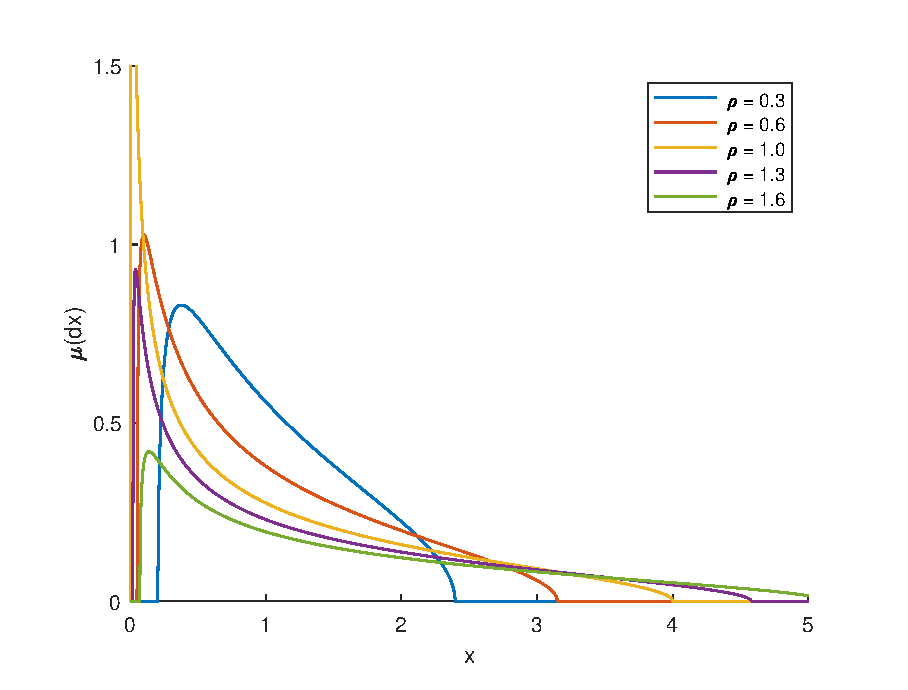
\includegraphics[width=\textwidth]{random-matrix-theory/figures/marchenko-pastur-distribution.eps}
        \caption{The Marčenko-Pastur Distribution}
    \end{subfigure}
    \begin{subfigure}{.49\linewidth}
        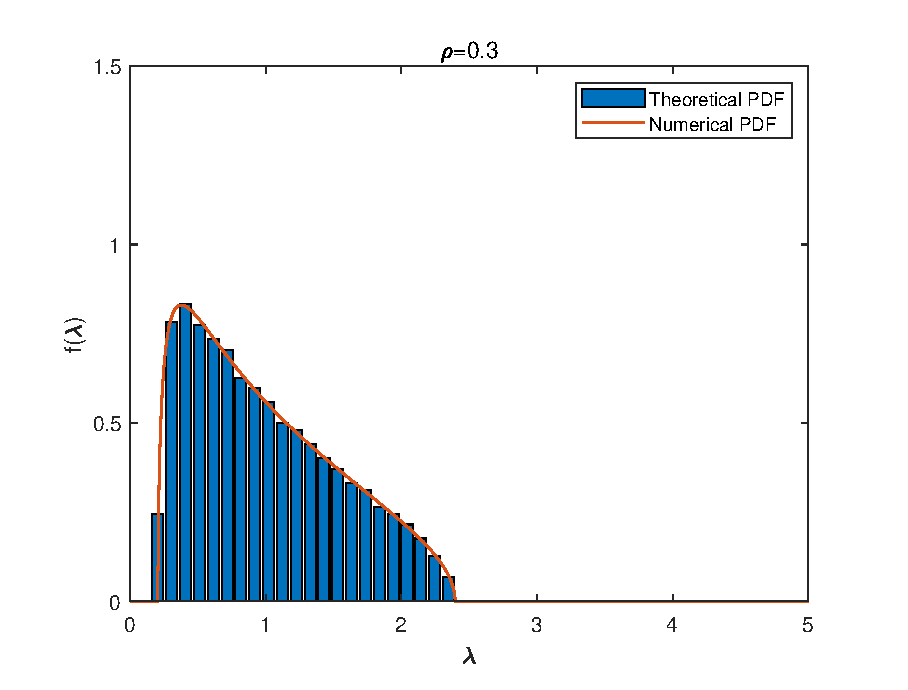
\includegraphics[width=\textwidth]{random-matrix-theory/figures/marchenko-pastur-theorem-simulation.eps}
        \caption{Simulation of Marčenko-Pastur Theorem}
    \end{subfigure}
    \caption{Illustrations of Marčenko-Pastur Theorem}
\end{figure}

\begin{proof}
    \textbf{Intuitive Idea:}
    Suppose $\overline{\mathbf{Q}}(z)=\mathbf{F}(z)^{-1}$ for some matrix $\mathbf{F}(z)$. To prove $\overline{\mathbf{Q}}(z)$ to be a deterministic equivalent for $\mathbf{Q}(z)$, particularly,
    \begin{equation*}
        \frac{1}{n}\operatorname{tr}\mathbf{A}(\mathbf{Q}(z)-\overline{\mathbf{Q}}(z))\rightarrow 0\quad\text{a.s.}
    \end{equation*}
    where $\mathbf{A}$ is arbitrary, deterministic, and such that $\|\mathbf{A}\|=1$. By Lemma \ref{lem:resolvent-identity}, we have
    \begin{equation*}
        \begin{aligned}
            \mathbf{Q}(z)-\overline{\mathbf{Q}}(z)= & \mathbf{Q}(z)\left(\mathbf{F}(z)+z\mathbf{I}_{n}-\widehat{\boldsymbol{\Sigma}}\right) \overline{\mathbf{Q}}(z)                                         \\
            =                                       & \mathbf{Q}(z)\left(\mathbf{F}(z)+z\mathbf{I}_{n}-\frac{1}{m_{n}}\sum_{i=1}^{m_{n}}\mathbf{X}_{i}\mathbf{X}_{i}^{\prime}\right)\overline{\mathbf{Q}}(z)
        \end{aligned}
    \end{equation*}
    Thus, we turn to prove that,
    \begin{equation*}
        \frac{1}{n}\operatorname{tr}\left[\left(\mathbf{F}(z)+z\mathbf{I}_{n}\right)\overline{\mathbf{Q}}(z)\mathbf{A}\mathbf{Q}(z)\right]-\frac{1}{n}\cdot\frac{1}{m_{n}}\sum_{i=1}^{m_{n}}\mathbf{X}_{i}^{\prime}\overline{\mathbf{Q}}(z)\mathbf{A}\mathbf{Q}(z)\mathbf{X}_{i}\rightarrow 0\quad\text{a.s.}
    \end{equation*}
    By Lemma \ref{lem:sherman-morrison}, we have
    \begin{equation*}
        \mathbf{Q}(z)\mathbf{X}_{i}=\frac{\mathbf{Q}_{-i}(z)\mathbf{X}_{i}}{1+\frac{1}{m_{n}}\mathbf{X}_{i}^{\prime}\mathbf{Q}_{-i}(z)\mathbf{X}_{i}}
    \end{equation*}
    where
    \begin{equation*}
        \mathbf{Q}_{-i}(z)=\left(\frac{1}{m_{n}}\sum_{j\neq i}\mathbf{X}_{j}\mathbf{X}_{j}^{\prime}-z\mathbf{I}_{n}\right)^{-1}
    \end{equation*}
    is independent of $\mathbf{X}_{i}$. By Lemma \ref{lem:quadratic-form-close-to-the-trace}, we have
    \begin{equation*}
        \frac{1}{n}\mathbf{X}_{i}^{\prime}\overline{\mathbf{Q}}(z)\mathbf{A}\mathbf{Q}(z)\mathbf{X}_{i}=\frac{\frac{1}{n}\mathbf{X}_{i}^{\prime}\overline{\mathbf{Q}}(z)\mathbf{A}\mathbf{Q}_{-i}(z)\mathbf{X}_{i}}{1+\frac{1}{m_{n}}\mathbf{X}_{i}^{\prime}\mathbf{Q}_{-i}(z)\mathbf{X}_{i}}\simeq\frac{\frac{1}{n}\operatorname{tr}\left[\overline{\mathbf{Q}}(z)\mathbf{A}\mathbf{Q}_{-i}(z)\right]}{1+\frac{1}{m_{n}}\operatorname{tr}\left[\mathbf{Q}_{-i}(z)\right]}
    \end{equation*}
    Hence, we need to prove the approximation that
    \begin{equation*}
        \frac{1}{n}\operatorname{tr}\left[\left(\mathbf{F}(z)+z\mathbf{I}_{n}\right)\overline{\mathbf{Q}}(z)\mathbf{A}\mathbf{Q}(z)\right]\simeq\frac{\frac{1}{n}\operatorname{tr}\left[\overline{\mathbf{Q}}(z)\mathbf{A}\mathbf{Q}(z)\right]}{1+\frac{1}{m_{n}}\operatorname{tr}\left[\mathbf{Q}(z)\right]}
    \end{equation*}
    If $\mathbf{F}(z)$ exist, for the approximation above to hold, $\mathbf{F}(z)$ must be of the type
    \begin{equation*}
        \mathbf{F}(z)\simeq\left(-z+\frac{1}{1+\frac{1}{m_{n}}\operatorname{tr}\mathbf{Q}(z)}\right)\mathbf{I}_{n}
    \end{equation*}
    By Equation \ref{eq:relation-between-empirical-spectral-measures-stieltjes-transform-and-its-resolvent}, we have,
    \begin{equation*}
        m(z)\equiv\frac{1}{n}\operatorname{tr}\left[\overline{\mathbf{Q}}(z)\right]=\frac{1}{n}\operatorname{tr}\left[\mathbf{F}(z)^{-1}\right]
    \end{equation*}
    taking $\mathbf{A}=\mathbf{I}_{n}$, we have
    \begin{equation*}
        \frac{1}{n}\operatorname{tr}\left[\mathbf{Q}(z)\right]\simeq\frac{1}{n}\operatorname{tr}\left[\overline{\mathbf{Q}}(z)\right]=m(z)=\frac{1}{-z+\frac{1}{1+\frac{n}{m_{n}}\frac{1}{n}\operatorname{tr}\left[\mathbf{Q}(z)\right]}}\simeq\frac{1}{-z+\frac{1}{1+\rho m(z)}}
    \end{equation*}
    As $n,m_{n}\rightarrow\infty$, $m(z)$ is solution to
    \begin{equation*}
        m(z)=\frac{1}{-z+\frac{1}{1+\rho m(z)}}
    \end{equation*}
    or equivalently
    \begin{equation*}
        z\rho m^{2}(z)-(1-\rho-z)m(z)+1=0
    \end{equation*}
    This equation has two solutions defined via the two values of the complex square root function. Let
    \begin{equation*}
        z=r\mathrm{e}^{\imath\theta}\text{ where }r\geq 0,\theta\in[0,2\pi)\Rightarrow\sqrt{z}\in\left\{\pm\sqrt{r}\mathrm{e}^{\imath\theta/2}\right\}
    \end{equation*}
    and we can conclude that
    \begin{equation*}
        m(z)=\frac{1-\rho-z}{2\rho z}+\frac{\sqrt{\left((1+\sqrt{\rho})^{2}-z\right)\left((1-\sqrt{\rho})^{2}-z\right)}}{2\rho z}
    \end{equation*}
    only one of which is such that $\Im[z]\Im[m(z)]>0$ as imposed by the definition of Stieltjes transforms. By the inverse Stieltjes transform theorem, Theorem \ref{thm:inverse-stieltjes-transform}, we find that $m(z)$ is the Stieltjes transform of the measure $\mu$ with
    \begin{equation*}
        \mu([a,b])=\frac{1}{\pi}\lim_{\epsilon\downarrow 0}\int_{a}^{b}\Im[m(x+\imath\epsilon)]\,\mathrm{d}x
    \end{equation*}
    for all continuity points $a,b\in\mathbb{R}$ of $\mu$. This term under the square root in $m(z)$ being negative only in the set
    \begin{equation*}
        \left[(1-\sqrt{\rho})^{2},(1+\sqrt{\rho})^{2}\right]
    \end{equation*}
    (and thus of non-real square root), the latter defines the support of the continuous part of the measure $\mu$ with density
    \begin{equation*}
        \frac{\sqrt{\left((1+\sqrt{\rho})^{2}-x\right)\left(x-(1-\sqrt{\rho})^{2}\right)}}{2\rho\pi x}
    \end{equation*}
    at point $x$ in the set. The case $x=0$ brings a discontinuity in $\mu$ with weight equal to
    \begin{equation*}
        \mu(\{0\})=-\lim_{y\downarrow 0}\imath ym(\imath y)=\frac{\rho-1}{2\rho}\pm\frac{\rho-1}{2\rho}
    \end{equation*}
    where the sign is established by a second order development of $z m(z)$ in the neighborhood of zero: that is, "+" for $c>1$ inducing a mass $1-1/\rho$ for $p>n$, or "-" for $c<1$ in which case $\mu(\{0\})=0$ and $\mu$ has no mass at zero.

    \textbf{Convergence in Mean:}
\end{proof}

\begin{remark}
    The asymptotic phenomenon holds not only in the Gaussian case, which also holds
    \begin{enumerate}
        \item if for every $n\in\mathbb{N}$ the distribution of the isotropic random vector $X_{n}$ is log-concave, where a probability measure $\mu$ on $\mathbb{R}^{n}$ with density $\varphi$ is log-concave when $\varphi=e^{-V}$ with $V$ convex.
        \item if $\left(X_{n,k}\right)_{n\geq 1,1\leq k\leq n}$ are i.i.d. with finite second moment.
    \end{enumerate}
\end{remark}

\section{Limits of Extreme Eigenvalues}

The weak convergence in Theorem \ref{thm:marcenko-pastur-theorem} does not provide much information at the edge on the behavior of the extremal atoms, and what one can actually extract is that
\begin{equation}
    \limsup_{n\rightarrow\infty}\lambda_{\min}\left(\widehat{\Sigma}_{n}\right)\leq(1-\sqrt{\rho})^{2}\leq(1+\sqrt{\rho})^{2}\leq\liminf_{n\rightarrow\infty}\lambda_{\max}\left(\widehat{\Sigma}_{n}\right),\quad\text{ a.s.}
\end{equation}
where the first inequality is considered only in the case where $m_{n}\geq n$.